%----------------------------------------------------------------------------------------
%   PACKAGES AND OTHER DOCUMENT CONFIGURATIONS
%----------------------------------------------------------------------------------------

\documentclass[12pt,a4paper,roman]{moderncv} % Font sizes: 10, 11, or 12; paper
% sizes: a4paper, letterpaper, a5paper, legalpaper, executivepaper or landscape; font families: sans or roman

\moderncvstyle{casual} % CV theme - options include: 'casual' (default),
% 'classic', 'oldstyle' and 'banking'
\moderncvcolor{blue} % CV color - options include: 'blue' (default), 'orange', 'green', 'red', 'purple', 'grey' and 'black'

\usepackage[portuguese]{babel}
\usepackage[scale=0.75]{geometry} % Reduce document margins
\usepackage{pdfpages}
\usepackage[utf8]{inputenc}
\usepackage{lscape}

%\setlength{\hintscolumnwidth}{3cm} % Uncomment to change the width of the dates column
%\setlength{\makecvtitlenamewidth}{10cm} % For the 'classic' style, uncomment to adjust the width of the space allocated to your name

%----------------------------------------------------------------------------------------
%   NAME AND CONTACT INFORMATION SECTION
%----------------------------------------------------------------------------------------
\renewcommand*{\namefont}{\fontsize{24}{29}\mdseries\upshape}
\firstname{Of\'icio} 
\familyname{11/2016} % Numero do oficio
\extrainfo{13Robotics Robotica LTDA -ME, CNPJ 17394264/0001-70}
\address{Rua Santa Alexandrina, 445}{Rio de Janeiro, RJ}
%\phone{(000) 111 1112}
%\fax{(000) 111 1113}
%\email{john@smith.com}
%\homepage{staff.org.edu/~jsmith}{staff.org.edu/$\sim$jsmith} % The first
% argument is the url for the clickable link, the second argument is the url displayed in the template - this allows special characters to be displayed such as the tilde in this example
\photo[200pt][0pt]{logo/logo.png} % The first bracket is the picture
% height, the second is the thickness of the frame around the picture (0pt for no frame)
\nopagenumbers
\linespread{1.25}
\begin{document}

\makecvtitle \textbf{Breno Bellinati de Carvalho\\
Gerente de Projeto\\
Energia Sustent\'avel do Brasil S. A. - ESBR}\hfill\\
\vspace{2mm}\\
\textbf{Prezados (as)},\hfill\\
\vspace{0.5mm}
% ----------------------------------------------------------------------------------------
% Corpo do oficio ---------------------------------------------------------

Solicitamos a aquisição de duas (2) passagens aéreas por parte da Energia Sustentável do Brasil S/A
para que os pesquisadores Eduardo Elael e Gabriel Alcantra da Thirteen Robotics possam estar em Porto Velho/RO no periódo de 07/11/2016 a 11/11/2016. O objetivo da viagem é participar do treinamento do fornecedor FARO no equipamento scaner laser de metrologia. O equipamento é utilizado no projeto EMMA II  (Prototipo para Revestimento Robótico de Turbinas In Situ) para se estimar a posição relativa entre o manipulador e a pá, após a montagem do manipulador no circuito hidráulico. 
Necessitamos que seja providenciado também aluguel de um (1) veículo para o deslocamento dos pesquisadores e dois (2) quartos de hotel durante o período de 07/11/2016 - 11/11/2016 
Solicitamos também que diárias de R\$ 300,00 para cada pesquisador sejam depositadas pela ESBR diretamente na conta do pesquisador: \\


\begin{itemize}  
\item R\$ 300,00 GABRIEL ALCANTARA COSTA SILVA	136.759.937-79	BANCO DO BRASIL 01	36528	49063-6 
\item R\$ 300,00 EDUARDO ELAEL DE MELO SOARES	045.287.677-08	BANCO DO BRASIL 01	19968	131161-1
\end{itemize}

\bigskip
 O valor de R\$ 300,00 é referente as diárias do: Dia 07/11/2016, translado residência-aeroporto e alimentação, valor de R\$ 150,00. Dia 11/11/2016, translado aeroporto-residência e alimentação, valor R\$ 150,00. Do dia 08/11/2016 ao 10/11/2016 não haverá pagamento de diária, pois a ESBR se responsabilizará pela hospedagem, transporte e alimentação dos pesquisadores. \\


Anexo I – Formulário de Atividades a Serem Executas.


% Assinatura ------------------------------------------------------------
\begin{center}

\includegraphics{patrick.png}\\ 
Patrick Paranhos\\
Rio de Janeiro, \today
\end{center}
%----------------------------------------------------------------------------------------

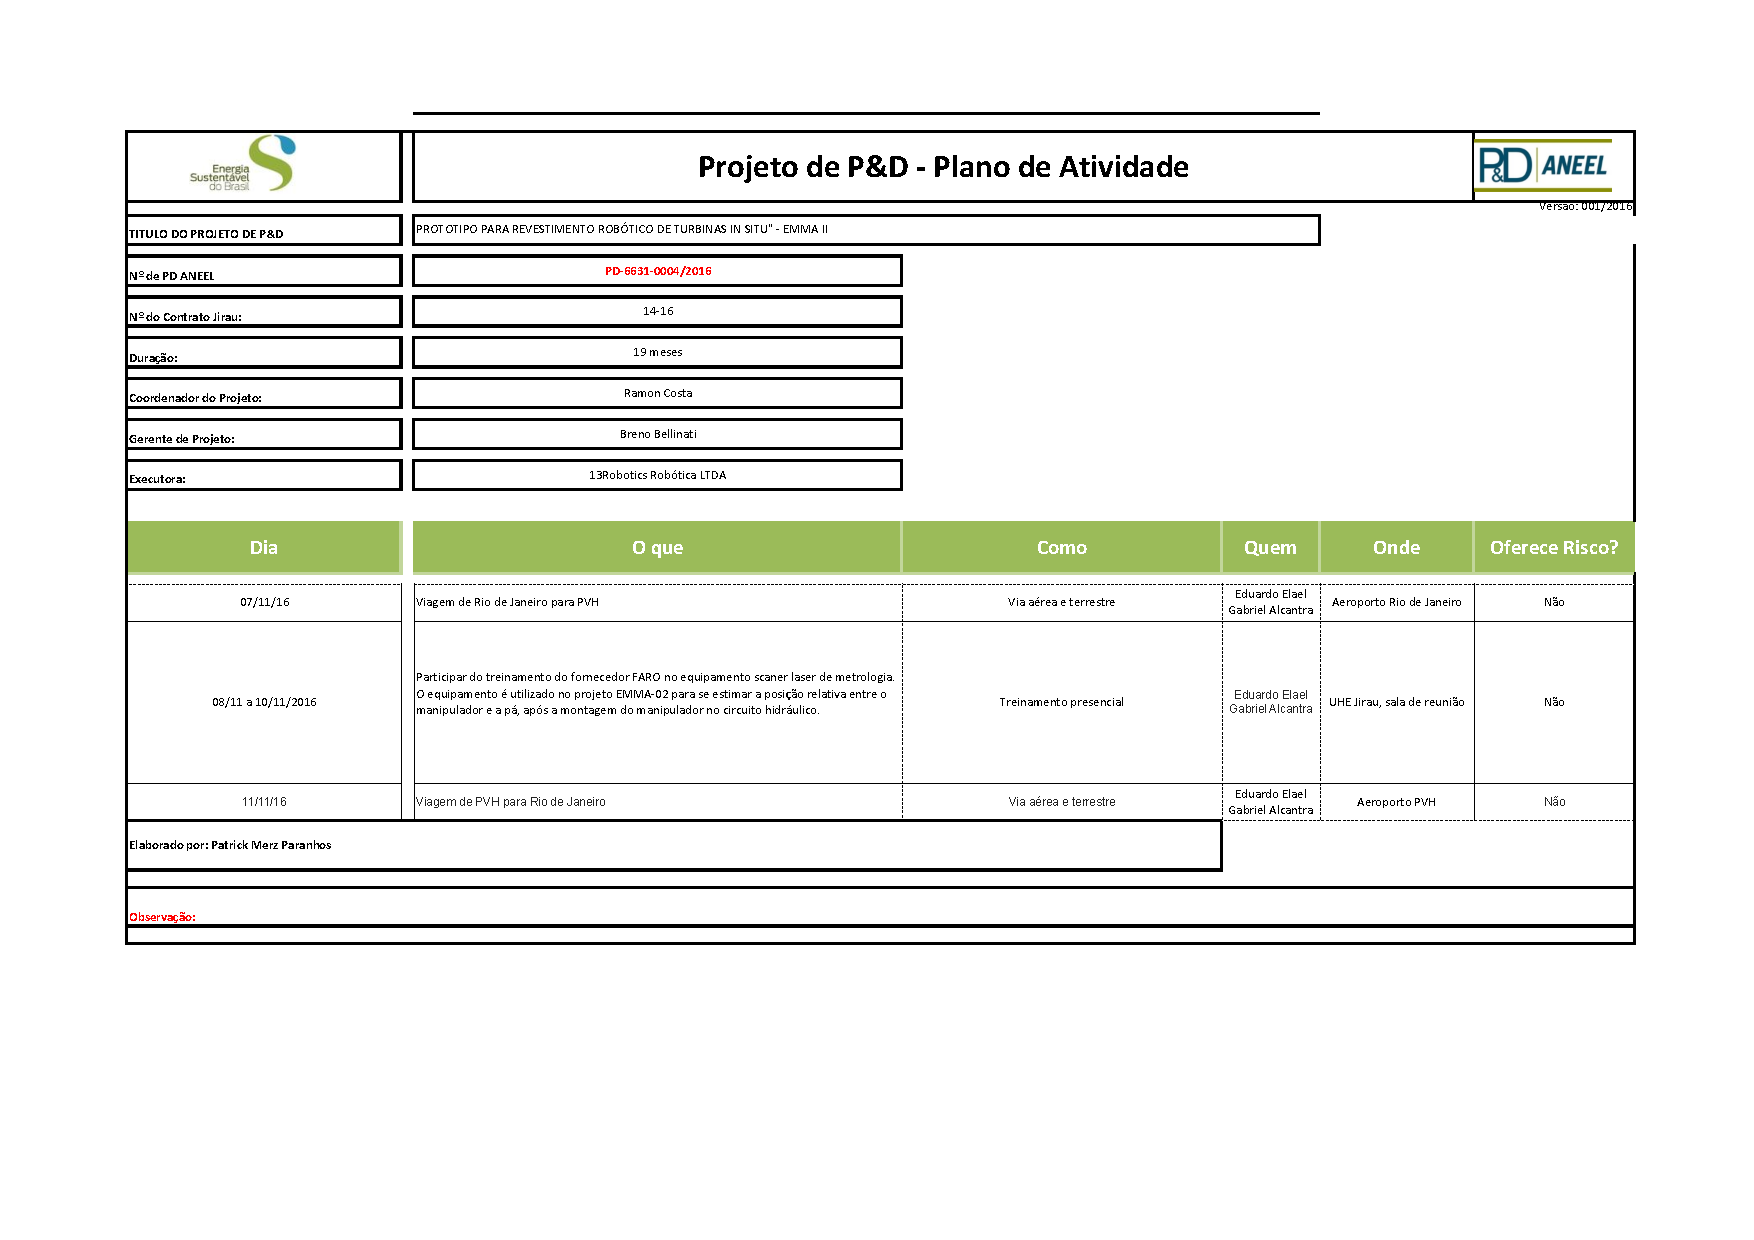
\includepdf[pages=-,pagecommand=\section{Anexo I}]{pdfs/atividade.pdf}

\end{document}